\documentclass[letterpaper,12pt]{article}

\usepackage{threeparttable}
\usepackage{geometry}
\geometry{letterpaper,tmargin=1in,bmargin=1in,lmargin=1.25in,rmargin=1.25in}
\usepackage[format=hang,font=normalsize,labelfont=bf]{caption}
\usepackage{amsmath}
\usepackage{mathrsfs}
\usepackage{multirow}
\usepackage{array}
\usepackage{delarray}
\usepackage{listings}
\usepackage{amssymb}
\usepackage{amsthm}
\usepackage{lscape}
\usepackage{natbib}
\usepackage{setspace}
\usepackage{float,color}
\usepackage[pdftex]{graphicx}
\usepackage{pdfsync}
\usepackage{verbatim}
\usepackage{placeins}
\usepackage{geometry}
\usepackage{pdflscape}
\synctex=1
\usepackage{hyperref}
\hypersetup{colorlinks,linkcolor=red,urlcolor=blue,citecolor=red}
\usepackage{bm}


\theoremstyle{definition}
\newtheorem{theorem}{Theorem}
\newtheorem{acknowledgement}[theorem]{Acknowledgement}
\newtheorem{algorithm}[theorem]{Algorithm}
\newtheorem{axiom}[theorem]{Axiom}
\newtheorem{case}[theorem]{Case}
\newtheorem{claim}[theorem]{Claim}
\newtheorem{conclusion}[theorem]{Conclusion}
\newtheorem{condition}[theorem]{Condition}
\newtheorem{conjecture}[theorem]{Conjecture}
\newtheorem{corollary}[theorem]{Corollary}
\newtheorem{criterion}[theorem]{Criterion}
\newtheorem{definition}{Definition} % Number definitions on their own
\newtheorem{derivation}{Derivation} % Number derivations on their own
\newtheorem{example}[theorem]{Example}
\newtheorem{exercise}[theorem]{Exercise}
\newtheorem{lemma}[theorem]{Lemma}
\newtheorem{notation}[theorem]{Notation}
\newtheorem{problem}[theorem]{Problem}
\newtheorem{proposition}{Proposition} % Number propositions on their own
\newtheorem{remark}[theorem]{Remark}
\newtheorem{solution}[theorem]{Solution}
\newtheorem{summary}[theorem]{Summary}
\bibliographystyle{aer}
\newcommand\ve{\varepsilon}
\renewcommand\theenumi{\roman{enumi}}
\newcommand\norm[1]{\left\lVert#1\right\rVert}

\begin{document}

\title{Math 320 Homework 3.6}
\author{Chris Rytting}
\maketitle

\subsection*{3.33}
Note that
\begin{align*}
    P \left( \left| \frac{B}{n} - p \right| \geq \varepsilon \right) &= P \left( \left| \frac{B}{n} - p \right|^2 \geq \varepsilon^2 \right) \\ 
    &\text{By Markov's Inequality, we have}\\
    &\leq  \frac{E \left[ \left( \frac{B}{n} - p \right)^2 \right]}{\varepsilon^2} \\
    &= \frac{E \left[ \left( \frac{B-pn}{n} \right)^2 \right]}{\varepsilon^2} \\
    &= \frac{\frac{1}{n^2}E \left[ \left( B-pn \right)^2 \right]}{\varepsilon^2} \\
    &= \frac{E \left[ \left( B-pn \right)^2 \right]}{n^2 \varepsilon^2} \\
    &= \frac{E \left[ B^2 - 2Bnp + (np)^2  \right]}{n^2 \varepsilon^2} \\
    &= \frac{E \left[ B^2 \right]-E\left[   2Bnp  \right] + E\left[(np)^2  \right]}{n^2 \varepsilon^2} \\
    &= \frac{E \left[ B^2 \right]-2npE\left[   B  \right] + E\left[(np)^2  \right]}{n^2 \varepsilon^2} \\
    &= \frac{E \left[ B^2 \right]-2E\left[   B  \right]E\left[   B  \right] + (np)^2}{n^2 \varepsilon^2} \\
    &= \frac{E \left[ B^2 \right]-2E\left[   B  \right]^2 + E\left[B  \right]^2}{n^2 \varepsilon^2} \\
    &= \frac{E \left[ B^2 \right]-E\left[   B  \right]^2 }{n^2 \varepsilon^2} \\
    &= \frac{\sigma_B^2}{n^2 \varepsilon^2} \\
    &\text{ and since $B$ is a binomial random variable, }\\
    &= \frac{p(1-p)}{n^2 \varepsilon^2} \\
    &\text{ and since $n \geq 1$}\\
    &\leq \frac{p(1-p)}{n \varepsilon^2} \\
\end{align*}

\subsection*{3.34}
The given equation, as $n \to \infty$,
\[P \left( \Big| \frac{1}{n} \sum^{n}_{i=1} X_i \Big| < \varepsilon \right) = 
P \left( \Big| \frac{X_1 + X_2 +\cdots+ X_n}{n} - 0 \Big| < \varepsilon\right) = 
P \left( \Big| \frac{X_1 + X_2 +\cdots+ X_n}{n} - \mu \Big| < \varepsilon\right)\]
is clearly the complement of the equation given for the Weak Law of Large Numbers so we have that, as $n \to \infty$

\[P \left( \Big| \frac{X_1 + X_2 +\cdots+ X_n}{n} - \mu \Big| \geq \varepsilon\right) + 
P \left( \Big| \frac{X_1 + X_2 +\cdots+ X_n}{n} - \mu \Big| < \varepsilon\right) = 1\]
Rearranging the inequality, and noting that as $n \to \infty$,

\[P \left( \Big| \frac{X_1 + X_2 +\cdots+ X_n}{n} - \mu \Big| \geq \varepsilon\right) = 0\] 
we have that


\[0 + 
P \left( \Big| \frac{X_1 + X_2 +\cdots+ X_n}{n} - \mu \Big| < \varepsilon\right) = 1\]
\[\implies P \left( \Big| \frac{X_1, + X_2 +\cdots+ X_n}{n} - \mu \Big| < \varepsilon\right) = 1\]

\subsection*{3.35}
Let $X_i$ be our random variable. By the Central Limit Theorem, we have that
\begin{align*}
    P( \sum^{n}_{i=1} X_i \leq 2000) &= P( \sum^{n}_{i=1}\frac{ X_i - n\mu }{\sqrt{n} \sigma}\leq \frac{ 2000 }{\sqrt{n} \sigma}) \\
    &= P( \sum^{n}_{i=1}\frac{ X_i - 10\cdot176 }{\sqrt{10} \cdot 30}\leq \frac{240}{\sqrt{10} \cdot 30}) \\
    &= P( \sum^{n}_{i=1}\frac{ X_i - 1760 }{\sqrt{10} \cdot 30}\leq \frac{240}{\sqrt{10} \cdot 30}) \\
\end{align*}
yielding
\[\frac{1}{\sqrt{2 \pi}} \int_{-\infty}^{\frac{240}{\sqrt{10}\cdot 30}} e^{-x^2/2} dx \approx .99429\]


\subsection*{3.36}

Let $X_i$ be our random variable. By the Central Limit Theorem, we have that
\begin{align*}
    P( \sum^{n}_{i=1} X_i \geq 5500) &= 1 - P( \sum^{n}_{i=1}\frac{ X_i - 6242\cdot.801 }{\sqrt{6242} \cdot.399428}\leq \frac{5500- 6242\cdot.801 }{\sqrt{6242}\cdot .399428}) \\
    &=1 -  P( \sum^{n}_{i=1}\frac{ X_i - 5000 }{\sqrt{6242}\cdot .399428}\leq \frac{500}{\sqrt{6242} \cdot.399428}) \\
\end{align*}
yielding
\[1 - \frac{1}{\sqrt{2 \pi}} \int_{-\infty}^{\frac{500}{\sqrt{6242}\cdot .399428}} e^{-x^2/2} dx \approx 2.22045\times10^{-16}\]




\subsection*{3.37}

Let $X_i$ be our random variable. Define it as follows:
\[
\begin{cases}
    1 & \text{if a 6 is rolled.}\\
    0 & \text{if otherwise.}\\
\end{cases}
\]
$p$, in this case, is $\frac{1}{6}$, and the variance is given by $p(1-p) = \frac{1}{6}\cdot\frac{5}{6} = \frac{\sqrt{5}}{6}$. By the Central Limit Theorem, we have that
\begin{align*}
    P\left( 150 \leq \sum^{n}_{i=1} X_i \leq 200 \right) &= P\left( \frac{150 - \frac{1}{6}900}{6\sqrt{900}\sqrt{5}} \leq \sum^{n}_{i=1} \frac{X_i - \frac{1}{6}900}{6\sqrt{900}\sqrt{5}} \leq \frac{200-\frac{1}{6}900}{6\sqrt{900}\sqrt{5}} \right) \\
    &= P\left( 0 \leq \sum^{n}_{i=1} \frac{X_i - 150}{5\sqrt{5}} \leq \frac{50}{5\sqrt{5}} \right) \\
\end{align*}
yielding
\[ \frac{1}{\sqrt{2 \pi}} \int_{0}^{\frac{50}{5\sqrt{5}}} e^{-x^2/2}dx \approx .499996\]

\subsection*{3.38}
\begin{lstlisting}
import numpy as np
from scipy import stats
import matplotlib.pyplot as plt
import matplotlib.mlab as mlab
import sys

#Problem 38
def Problem1(a,b):
    mean1, var1 = stats.beta.stats(a,b, moments='mv')
    x = np.linspace(stats.beta.ppf(.01,a,b), stats.beta.ppf(.99, a, b), 100)
    plt.plot(x,stats.beta.pdf(x,a,b))
    print "Mean: ", mean1,"\nVariance: ", var1
    vals = np.array([1,2,4,8,16,32])
    for i in vals:
        plt.plot(x,mlab.normpdf(x,mean1,np.sqrt(var1/i)))
        xbar = np.average(stats.beta.rvs(a,b,size=(i,1000)),axis = 0)
        plt.hist(xbar,normed=True)

Problem1(1,4)
plt.show()
Problem1(1,1)
plt.show()

OUTPUT

Mean:  0.2
Variance:  0.0266666666667
Mean:  0.5
Variance:  0.0833333333333
\end{lstlisting}
\[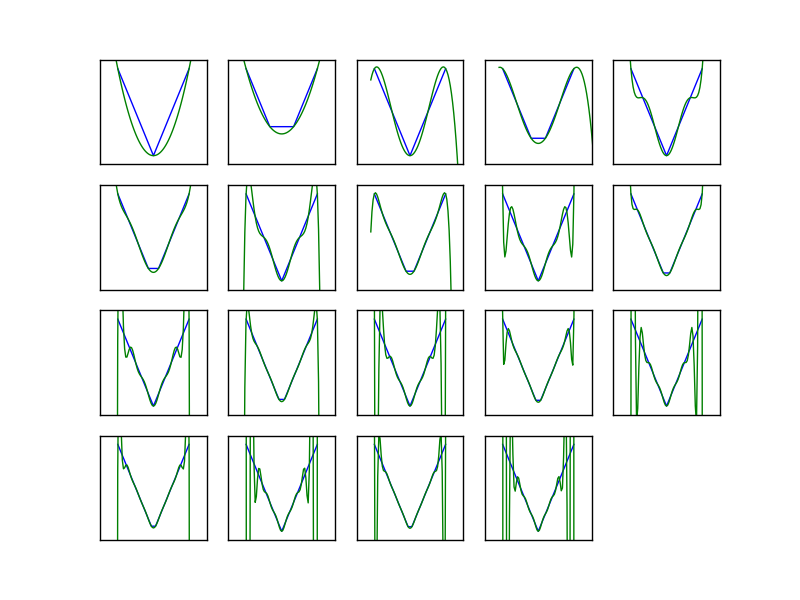
\includegraphics[scale = .7]{figure1.png}\]
\[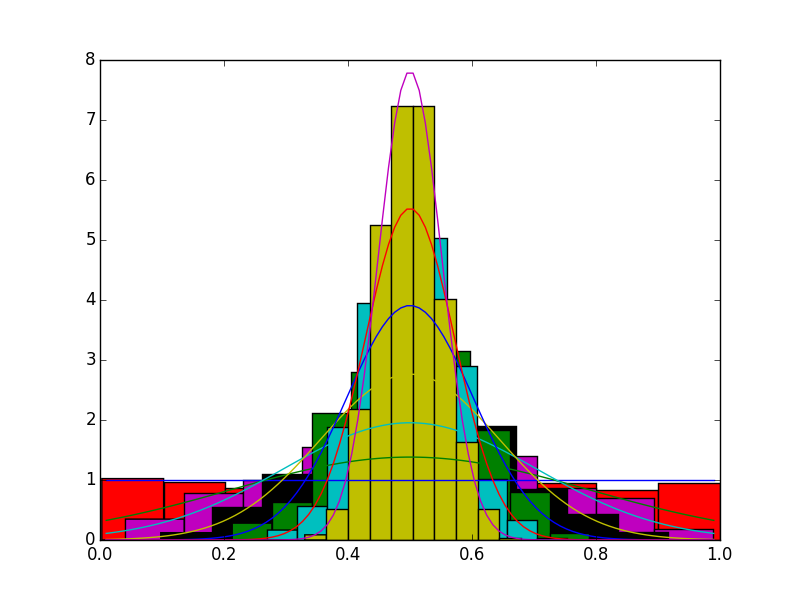
\includegraphics[scale = .7]{figure2.png}\]






\end{document}
